% !TeX root = ../../Book2.tex
% 纲要标题：## 第16章　映射度、相交与局部指标
% 纲要位置：几何学计划纲要.md，第 1621 行。
% 正文状态：初稿；尚未正式审核。

% 纲要内容开始
% 
% > 本章目标与证明范围：用横截性把代数对偶解释为几何计数，再以一维配边证明不变性。所有整数计数有明确取向规则，非横截情形通过扰动而非朴素点数处理。
% 
% 纲要内容结束

\chapter{映射度、相交与局部指标}
\label{g2:ch:16}
\BookChapterNumber{g2:ch:16}

\begin{chapterabstract}
	正则值的带符号原像数、子流形的相交数、向量场零点指标和不动点指数，都把局部方向信息汇成整数。本章比较映射度的正则值、同调及积分定义，说明固有性如何控制非紧情形；用横截扰动和有向一维配边构造相交数，并与帽积配对比较。局部球面度给出向量场指标及其可加性，截面同伦则保持闭流形上的总指标。最后把不动点看作图像与对角线的交点，计算对角类，得到局部指数之和等于上同调交错迹的 Lefschetz 公式。
\end{chapterabstract}

\begin{learninggoals}
	\begin{itemize}
		\item 由正则值的微分符号计算映射度，并证明它与基本类及顶次形式积分的计算一致。
		\item 核对非紧映射的固有性、形式的紧支集及同伦的整体固有性，判断度公式何时适用。
		\item 按法向优先约定确定相交符号，用一维配边证明扰动不变性，并把交点计数写成帽积配对。
		\item 由小球边界的方向度计算孤立零点指标，证明坐标无关性、非退化公式及扰动后的可加性。
		\item 用截面横截同伦比较闭流形上不同向量场的总指标，并区分局部指标与零点个数。
		\item 从图像、对角类和杯积符号推导 Lefschetz 公式，由非零 Lefschetz 数判定不动点的存在。
	\end{itemize}
\end{learninggoals}

方程 \(x^3-x=0\) 有三个实根 \(-1,0,1\)，函数在这些点的导数分别为 \(2,-1,2\)。若只数根，答案是3；若同时记录穿过目标值的方向，答案则是 \(1-1+1=1\)。把右端换成充分大的正数，方程只有一个实根，导数为正，带符号的答案仍然是1。原像点会出现或消失，方向计数却保留了一个稳定的整数。

\ProseParagraphBreak

同样的现象也出现在曲线相交、向量场零点与不动点问题中。两条曲线相切后可能产生两个交点；一个退化零点可能裂成多个非退化零点；一个自映射的不动点可以随着映射改变而移动。把这些现象放进一参数族，满足横截条件的全部解组成一维流形，其边界记录初、末状态。方向规定使区间的两个端点贡献相反符号，这便是计数保持不变的几何原因。

\ProseParagraphBreak

\secref{g2:sec:1601}先把这种计数与第3章的局部度、第6章的基本类和第7章的积分比较连接起来。\secref{g2:sec:1602}将目标点换成子流形，比较相交符号与法向方向，再证明几何交数等于相应的对偶配对。\secref{g2:sec:1603}考察向量场在小球边界上的朝向，得到能容纳退化零点的指标。\secref{g2:sec:1604}则把方程 \(f(x)=x\) 写成图像与对角线相交，从局部的 \(\det(I-\mathrm{d}f_x)\) 走到上同调上的交错迹。

\ProseParagraphBreak

本章使用第4章的外积与杯积符号、第6章的帽积和 Poincaré 对偶，以及第14章的相对横截性和第15章的管状邻域。关键调用处会恢复定向、维数、紧性及支集条件：它们决定交集是否有限、符号能否连续选择，以及一族解是否会逃到无穷远。正则值与积分度的比较可参阅\cite[第457--459页，定理17.35及命题17.36]{Lee2012Smooth}；有限复形及其回缩空间的 Lefschetz 定理可参阅\cite[第2.C节，The Lefschetz Fixed Point Theorem]{Hatcher2002}。

% !TeX root = ../../Book2.tex
% 纲要标题：### 16.1 映射度的等价定义
% 纲要位置：几何学计划纲要.md，第 1625 行。
% 正文状态：初稿；尚未正式审核。

% 纲要内容开始
% 
% * 正则值处的局部符号
% * 同调定义与积分定义的比较
% * 固有映射的映射度
% * 复合公式及典型计算
% 
% 纲要内容结束

\section{映射度的等价定义}
\label{g2:sec:1601}

圆周映射 \(z\mapsto z^k\) 的度既可以从顶维同调读出，也可以在一个目标点处数原像，还可以由角形式的积分求得。这三个计算测量的是同一件事：源流形按方向把目标覆盖了多少次。对一般流形，临界点会使覆盖片出现、合并或消失，非紧源还允许原像逃到无穷远。本节先解释每个正则原像的符号，再证明三种度的一致性，并把无穷远处所需的条件写清楚。除另有说明，流形均有限维、Hausdorff、第二可数。

\subsection{正则值处的局部符号}
\label{g2:subsec:1601:01}

设 \(f:M^n\to N^n\) 为定向无边界光滑流形间的光滑映射，\(n\ge1\)。若 \(y\) 是正则值，则每个 \(x\in f^{-1}(y)\) 处的微分 \(\mathrm{d}f_x\) 是同构。在源、目标各取一组正向基，定义
\[
	\varepsilon_x(f)=\operatorname{sgn}\det(\mathrm{d}f_x)\in\{1,-1\}.
\]
更换正向基只会让行列式乘以正数，因此该符号与基无关。它记录这一小片是保持方向还是反转方向，不能用行列式的绝对值替代。

\begin{proposition}\label{g2:prop:regular-local-degree-sign}
	设 \(f:M^n\to N^n\) 为定向无边界光滑流形间的光滑映射，\(n\ge1\)，且 \(\mathrm{d}f_x\) 可逆。按定向局部同调生成元定义的局部度满足
	\[
		\deg_x(f)=\varepsilon_x(f).
	\]
	若 \(f\) 固有，则每个正则值的原像有限。
\end{proposition}
\begin{proof}
	\cref{g2:def:local-degree}中的空间对定义可直接用于定向流形：由坐标切除，\(H_n(M,M\setminus\{x\};\mathbb Z)\cong\mathbb Z\)，其正生成元由定向指定。在正向坐标中把 \(x,f(x)\) 移到原点，写 \(f(z)=Az+r(z)\)，其中 \(A=\mathrm{d}f_x\) 可逆、\(|r(z)|/|z|\to0\)。取 \(c>0\) 使 \(|Az|\ge c|z|\)，再把坐标球缩小，使 \(|r(z)|<c|z|/2\)。于是
	\[
		|Az+s r(z)|\ge c|z|/2>0\qquad(z\ne0,\ 0\le s\le1).
	\]
	这给出穿孔空间对上的同伦，所以局部度等于线性映射 \(A\) 的局部度。

	对可逆矩阵作 Gram--Schmidt 分解，上三角部分可在保持对角元为正时连续变为恒等；正交部分则用平面旋转化为恒等，或化为一次坐标反射，分别对应 \(\det A>0\) 与 \(\det A<0\)。这些变化始终保持可逆，故仍是穿孔空间对同伦。恒等映射保持局部生成元，反射使其变号：通过相对球与边界球的连接同构，这正是\cref{g2:prop:reflection-antipodal-degree}已证的反射度。于是局部度为 \(\operatorname{sgn}\det A\)。

	第一卷第11章第3节的逆函数定理又说明正则原像的每个点都孤立。若 \(f\) 固有，纤维 \(f^{-1}(y)\) 是紧集；紧离散集有限，得到最后一项。
\end{proof}

对固有 \(f\) 及其正则值 \(y\)，可以先记带符号计数
\[
	d_y(f)=\sum_{x\in f^{-1}(y)}\varepsilon_x(f),
\]
空原像对应空和0。\cref{g2:thm:sard}保证存在正则值。为什么在变形时要数正负号，而不只数点数？一条有向的一维逆像会把新生或消失的两个端点赋予相反符号。

\begin{proposition}\label{g2:prop:oriented-regular-fiber-cobordism}
	设 \(M^n\) 为紧定向无边界光滑流形，\(N^n\) 为定向无边界光滑流形，\(n\ge1\)。若光滑映射 \(f_0,f_1:M\to N\) 同伦，且 \(y\in N\) 同时为两者的正则值，则 \(d_y(f_0)=d_y(f_1)\)。
\end{proposition}
\begin{proof}
	\cref{g2:thm:transverse-homotopy-cobordism}给出光滑同伦 \(H:M\times[0,1]\to N\)，在两端的时间邻域分别等于 \(f_0,f_1\)，并横截于 \(\{y\}\)。因 \(M\) 紧，\(W=H^{-1}(y)\) 是紧一维带边界流形，边界为两个端点纤维。

	这里给 \(M\times[0,1]\) 取 \(M\) 的方向在前、时间方向在后的乘积定向。给 \(W\) 的取向规定如下：先取 \(\mathrm{T}_yN\) 的正向基，选它们经 \(\mathrm{d}H\) 的任意提升，再接一条 \(\mathrm{T}W\) 的正向基，所得应是环境的正向基。这就是商方向在前、核方向在后的约定；改变提升只添加核方向，不改变取向。

	在端点附近，\(H(x,t)=f_j(x)\)，故 \(\partial_t\) 张成核。提升目标正向基到 \(\mathrm{T}_xM\) 后，其相对 \(M\) 的符号为 \(\varepsilon_x(f_j)\)，所以 \(W\) 的正向切向量是 \(\varepsilon_x(f_j)\partial_t\)。按照外法向优先的边界定向，\(t=1\) 端点的符号是 \(\varepsilon_x(f_1)\)，\(t=0\) 端点的符号是 \(-\varepsilon_x(f_0)\)。第一卷第14章第4节的 Stokes 定理对 \(W\) 上常函数1给出
	\[
		0=\int_W\mathrm{d}1=\int_{\partial W}1
		=d_y(f_1)-d_y(f_0).
	\]
	因而两个带符号计数相等。
\end{proof}

\subsection{同调定义与积分定义的比较}
\label{g2:subsec:1601:02}

第3章对球面定义的度可以原样推广到连通闭定向流形。这里“闭”仍表示紧且无边界。\cref{g2:thm:fundamental-class}给出由定向确定的正生成元 \([M]\in H_n(M;\mathbb Z)\) 与 \([N]\in H_n(N;\mathbb Z)\)。对连续映射 \(f:M\to N\)，唯一满足
\begin{equation}\label{g2:eq:manifold-homological-degree}
	f_*[M]=(\deg f)[N]
\end{equation}
的整数称为 \(f\) 的映射度。这个定义已说明同伦不变性；还须证明正则值计数和积分确实产生这一整数。

\ProseParagraphBreak

比较积分时，一个容易被略过的环节是：在基本类上对积分上链求值，为什么等于通常的流形积分？第7章给出了形式与奇异上同调的积分比较，下面用坐标盒中的基本类补足这一识别，也同时准备非紧情形所需的支集版本。

\begin{lemma}\label{g2:lem:integration-fundamental-pairing}
	设 \(M^n\) 为定向无边界光滑流形，\(n\ge1\)，\(\omega\in\Omega_c^n(M)\)。以 \([M]_{\mathrm{lf}}\) 表示与该定向对应的局部有限基本类，则
	\[
		\bigl\langle\mathcal I_{c,M}[\omega],[M]_{\mathrm{lf}}\bigr\rangle
		=\int_M\omega.
	\]
	左端的求值先在包含 \(\operatorname{supp}\omega\) 的紧集上相对化；若 \(M\) 闭，它就是通常的上同调与基本类配对。
\end{lemma}
\begin{proof}
	\cref{g2:thm:de-rham-support}把紧支形式的积分解释为紧支上同调类。若支集包含于紧集 \(K\)，这个上链在完全落入 \(M\setminus K\) 的单形上为零，因此可对 \([M]_K\) 求值；\cref{g2:prop:lf-fundamental-class}说明 \([M]_{\mathrm{lf}}\) 的相对化恰为 \([M]_K\)。

	先设 \(\omega\) 的支集紧含于一张正向坐标盒的内部。在该图域内取一个内部包含支集的闭盒，将它按正向仿射单形剖分，所得有限光滑链 \(c\) 的边界避开支集。在支集的每一点，\(c\) 的局部同调值都是正生成元；由\cref{g2:lem:compact-localization}的唯一性，\(c\) 表示该支集上的基本类。于是积分上链的定义及有限可加性给出
	\[
		\langle I\omega,c\rangle=\sum_{\sigma\text{ 为盒中单形}}\int_\sigma\omega
		=\int_M\omega.
	\]
	对于一般紧支 \(\omega\)，用有限张较小正向坐标盒覆盖支集，并以从属光滑单位分解写成有限和 \(\omega=\sum_\alpha\omega_\alpha\)，每项都紧支于相应盒内。对每项应用刚才的计算，再用配对和积分的线性性相加即得结论。
\end{proof}

\begin{theorem}[映射度比较定理]\label{g2:thm:degree-comparison}
	设 \(M,N\) 为连通闭定向光滑 \(n\) 维流形，\(n\ge1\)，\(f:M\to N\) 光滑。则对每个正则值 \(y\in N\)，
	\begin{equation}\label{g2:eq:degree-regular-value}
		\deg f=\sum_{x\in f^{-1}(y)}\operatorname{sgn}\det(\mathrm{d}f_x).
	\end{equation}
	对每个光滑顶次形式 \(\omega\in\Omega^n(N)\)，还有
	\begin{equation}\label{g2:eq:degree-integral}
		\int_M f^*\omega=(\deg f)\int_N\omega.
	\end{equation}
	因此正则值计数与正则值的选择无关；任取 \(\int_N\eta=1\) 的顶次形式，积分 \(\int_Mf^*\eta\) 都等于上述同调度。
\end{theorem}
\begin{proof}
	紧源使 \(f\) 固有，故 \(F=f^{-1}(y)\) 有限。先比较基本类在这些点附近的像。切除给出
	\[
		H_n(M,M\setminus F;\mathbb Z)
		\cong\bigoplus_{x\in F}H_n(M,M\setminus\{x\};\mathbb Z),
	\]
	并把 \([M]\) 的限制送到各局部正生成元组成的向量。与第3章的局部度求和相同，空间对映射给出交换图
	\[
		\begin{tikzcd}[column sep=large,row sep=large]
			H_n(M;\mathbb Z) \arrow[r] \arrow[d,"f_*"'] & \displaystyle\bigoplus_{x\in F}H_n(M,M\setminus\{x\};\mathbb Z) \arrow[d,"\sum f_{*,x}"] \\
			H_n(N;\mathbb Z) \arrow[r] & H_n(N,N\setminus\{y\};\mathbb Z).
		\end{tikzcd}
	\]
	沿左、下两边，\([M]\) 变为 \((\deg f)[N]_y\)；沿上、右两边，\cref{g2:prop:regular-local-degree-sign}给出 \(\sum_{x\in F}\varepsilon_x(f)[N]_y\)。右侧每个局部箭头先经切除取到只含这一个原像点的小邻域，再由 \(f\) 的限制诱导。比较系数即得\eqref{g2:eq:degree-regular-value}。若 \(F\) 为空，上方相对群为零，同一论证给出度为零。

	所有顶次形式都闭。由\cref{g2:lem:integration-fundamental-pairing,g2:prop:integration-naturality}及上同调求值的自然性，
	\begin{align*}
		\int_Mf^*\omega
		&=\bigl\langle\mathcal I_M[f^*\omega],[M]\bigr\rangle
		=\bigl\langle f^*\mathcal I_N[\omega],[M]\bigr\rangle\\
		&=\bigl\langle\mathcal I_N[\omega],f_*[M]\bigr\rangle
		=(\deg f)\int_N\omega.
	\end{align*}
	最后，在一张正向坐标图内取非负、非零的紧支顶次形式，再除以其正积分，就得到 \(\int_N\eta=1\) 的形式。因此积分的倍数唯一，且已由基本类证明为整数。
\end{proof}

这个证明补全了第一卷第14章第5节预先陈述的次数积分公式。维数0时，连通闭流形只有一个点，基本类记录该点的定向符号，积分就是带符号求值，同一公式直接成立。积分表达适用于所有顶次形式，包括积分为零的形式；只有把度写成两个积分之比时，才要求分母非零。局部微分给出的正负号决定同调中的整数，而积分把这个整数读成拉回后的总量。正则值与积分的比较也见\cite[第457--459页，定理17.35及命题17.36]{Lee2012Smooth}。

\subsection{固有映射的映射度}
\label{g2:subsec:1601:03}

连通非紧流形的普通顶次同调为零，见\cref{g2:prop:noncompact-top-homology}。因此把\eqref{g2:eq:manifold-homological-degree}中的普通基本类照搬过去，会失去要计数的信息。第6章的局部有限链允许沿整个流形延伸，只要求每个紧集遇到有限项；其基本类仍在每一点具有正的局部值。

\begin{definition}\label{g2:def:proper-manifold-degree}
	设 \(M,N\) 为连通定向无边界光滑 \(n\) 维流形，\(n\ge1\)，\(f:M\to N\) 为固有连续映射。由
	\[
		f_*[M]_{\mathrm{lf}}=(\deg f)[N]_{\mathrm{lf}}
	\]
	确定的整数称为 \(f\) 的映射度。这里使用整数系数的局部有限同调。
\end{definition}

这个定义的两个依据需要同时保留。\cref{g2:thm:poincare-duality-locally-finite}在次数0给出 \(H_n^{\mathrm{lf}}(N;\mathbb Z)\cong H^0(N;\mathbb Z)=\mathbb Z\)，基本类对应1。另一方面，\cref{g2:prop:support-functoriality}中的固有性使推前有定义：目标紧集 \(K\) 的逆像紧，故原局部有限链只有有限条单形可能在推前后遇到 \(K\)。若 \(M,N\) 都闭，这一定义就是前面的普通同调度。

\begin{theorem}[固有映射的度公式]\label{g2:thm:proper-degree-formulas}
	设 \(f:M^n\to N^n\) 为连通定向无边界光滑流形间的固有光滑映射，\(n\ge1\)。对任一正则值 \(y\) 及任一紧支顶次形式 \(\omega\in\Omega_c^n(N)\)，有
	\[
		\deg f=\sum_{x\in f^{-1}(y)}\operatorname{sgn}\det(\mathrm{d}f_x),
		\qquad \int_Mf^*\omega=(\deg f)\int_N\omega.
	\]
	特别地，非零度强迫 \(f\) 满射。
\end{theorem}
\begin{proof}
	正则纤维紧且离散，因而有限。将局部有限基本类相对化到 \(f^{-1}(y)\) 与 \(\{y\}\)，得到与\cref{g2:thm:degree-comparison}相同的交换图；各局部值仍是正生成元，故得到符号求和公式。

	固有性保证 \(\operatorname{supp}f^*\omega\subset f^{-1}(\operatorname{supp}\omega)\) 紧。由\cref{g2:thm:de-rham-support}的固有拉回相容性，\(\mathcal I_{c,M}[f^*\omega]=f^*\mathcal I_{c,N}[\omega]\)。紧支上链与局部有限链的求值满足
	\[
		\langle f^*a,c\rangle=\langle a,f_*c\rangle;
	\]
	两边实际都只涉及支集附近的有限项，逐单形就是同一项。再用\cref{g2:lem:integration-fundamental-pairing}和度的定义，得到积分公式。若 \(y\) 不在像内，它自动是正则值，空和公式便给出 \(\deg f=0\)。
\end{proof}

同伦也须保留无穷远处的控制。设 \(H:M\times[0,1]\to N\) 是连续同伦；称它为固有同伦，是指这个整体映射固有。它使两个端点在局部有限同调上的推前相同。为验证这一点，对局部有限链逐项使用\cref{g2:thm:singular-homotopy-invariance}的棱柱算子。若某个输出棱柱遇到目标紧集 \(K\)，原单形必遇到紧集
\[
	\operatorname{pr}_M\bigl(H^{-1}(K)\bigr).
\]
这样的原单形只有有限条，每条棱柱又只剖成有限个单形，所以棱柱算子仍局部有限，原来的等式 \(\partial P+P\partial=H_{1\#}-H_{0\#}\) 继续成立。因此固有同伦保持映射度。

\begin{example}\label{g2:exm:proper-slices-not-proper-homotopy}
	对 \(0\le t\le1\) 令 \(H_t:\mathbb R\to\mathbb R\)、\(H_t(x)=x+t x^2\)。每个固定时刻的映射都固有：\(t=0\) 时为恒等，\(t>0\) 时二次项使函数在两端趋于正无穷。值0对每张切片都是正则值。\(t=0\) 时只有原像0、符号为正，故度为1；\(t>0\) 时原像为 \(0,-1/t\)，导数分别为 \(1,-1\)，故度为0。

	整体同伦并不固有，因为 \(H^{-1}(0)\) 包含 \((-1/t,t)\)，当 \(t\downarrow0\) 时这些点逃向无穷远。两条相反符号的分支中有一条从无穷远进入，正好说明“每张切片固有”不能代替“整个同伦固有”。
\end{example}

连映射本身都不固有时，正则值计数也可能随位置改变。例如 \(f:\mathbb R\to\mathbb R\)、\(f(x)=e^x\)，每个正数有一个符号为正的原像，每个负数没有原像。其像未覆盖零点附近的负半轴，而趋向0的原像跑向负无穷。积分虽对某些拉回仍收敛，也不能据此指定统一的度：\(\int_{\mathbb R}f^*(a(y)\,\mathrm{d}y)=\int_0^\infty a(y)\,\mathrm{d}y\)，随紧支函数 \(a\) 在正、负半轴间的分布变化，无法等于一个固定整数乘 \(\int_{\mathbb R}a(y)\,\mathrm{d}y\)。

\subsection{复合公式及典型计算}
\label{g2:subsec:1601:04}

\begin{proposition}\label{g2:prop:manifold-degree-laws}
	设 \(M,N,P\) 为连通定向无边界光滑 \(n\) 维流形，\(n\ge1\)，\(f:M\to N\)、\(g:N\to P\) 固有连续。则
	\[
		\deg(g\circ f)=(\deg g)(\deg f),\qquad\deg(\operatorname{id}_M)=1.
	\]
	保定向微分同胚的度为1，反定向微分同胚的度为 \(-1\)。反转源或目标其中一端的定向使度变号，同时反转两端则不变。
\end{proposition}
\begin{proof}
	固有映射的复合仍固有，局部有限推前满足复合律，所以
	\[
		(gf)_*[M]_{\mathrm{lf}}
		=g_*\bigl((\deg f)[N]_{\mathrm{lf}}\bigr)
		=(\deg f)(\deg g)[P]_{\mathrm{lf}}.
	\]
	恒等映射保持基本类。微分同胚是固有映射，每个目标点只有一个正则原像，符号求和公式给出 \(\pm1\)。定向反转使对应基本类乘以 \(-1\)，代入定义即得最后一项。
\end{proof}

若 \(p:M\to N\) 是连通定向流形间的 \(r\) 层光滑覆盖，且局部微分保持定向，则 \(\deg p=r\)；若处处反向，则 \(\deg p=-r\)。有限层覆盖在流形间固有：目标紧集可由有限个闭包位于均匀覆盖邻域的小坐标块覆盖，每块的全部原像是有限个紧块。局部符号在连通源上恒定，故上面两个结论直接由每个纤维的 \(r\) 项求和得到。圆周 \(z\mapsto z^k\) 的度 \(k\) 是这一计算的一维例子。

\begin{example}\label{g2:exm:torus-integer-matrix-degree}
	令 \(T^n=\mathbb R^n/\mathbb Z^n\)，取标准定向。对整数矩阵 \(A\in\operatorname{Mat}_{n\times n}(\mathbb Z)\)，映射
	\[
		f_A([x])=[Ax]
	\]
	良定义。形式 \(\eta=\mathrm{d}x^1\wedge\cdots\wedge\mathrm{d}x^n\) 在整数平移下不变，因而下降到环面，且 \(\int_{T^n}\eta=1\)。直接计算 \(f_A^*\eta=(\det A)\eta\)，所以
	\[
		\deg f_A=\det A.
	\]
	例如 \(A=\begin{pmatrix}2&1\\0&-3\end{pmatrix}\) 给出度 \(-6\)。若 \(\det A\ne0\)，每个点都是正则点，各原像点的符号均为 \(\operatorname{sgn}\det A\)，所以符号求和公式说明每个纤维有 \(|\det A|\) 个点；若 \(\det A=0\)，积分拉回为零，度也为零。行列式同时包含覆盖片数与方向，两者在这一模型中恰好合为一个整数。
\end{example}

\begin{example}\label{g2:exm:antipodal-differential-degree}
	给 \(S^n\subset\mathbb R^{n+1}\) 取外法向优先定向，对径映射 \(a(x)=-x\) 的度为 \((-1)^{n+1}\)，与第3章的同调计算相同。若 \((x,v_1,\ldots,v_n)\) 是环境中的正向基，映射后的外法向是 \(-x\)，切向量为 \(-v_i\)。整个 \(n+1\) 元组乘以 \(-1\)，故其符号为 \((-1)^{n+1}\)。这就是 \(\mathrm{d}a_x\) 相对于源、目标球面定向的符号。直接把它看作“\(n\) 个切向量都变负”会漏掉目标点的外法向也已改变这一事实。
\end{example}

度不等于未经加权的覆盖次数。例如 \(p(x)=x^3-x\) 是实线到实线的固有映射；在正则值0上有三个原像 \(-1,0,1\)，导数符号为 \(+,-,+\)，因此度为1。在充分大的正则值上只有一个原像，符号仍为正。临界值两侧原像数变化，代数和却保持不变。

% !TeX root = ../../Book2.tex
% 纲要标题：### 16.2 相交数的构造
% 纲要位置：几何学计划纲要.md，第 1632 行。
% 正文状态：初稿；尚未正式审核。

% 纲要内容开始
% 
% * 互补维子流形的线性取向
% * 横截扰动与零维交集
% * 一参数族给出的配边
% * 交数与帽积配对的比较
% 
% 纲要内容结束

\section{相交数的构造}
\label{g2:sec:1602}

环面上的一条经线和一条纬线相交一次；把其中一条弯曲，可能额外出现两个交点，却仍不能把两条曲线彻底分开。记录每次穿过的方向后，新出现的两个交点符号相反，计数因而保持不变。第6章用杯积与基本类定义了代数配对，本节将证明，这个配对正是几何中的带符号交点数。先明确局部符号，再用横截扰动与一维配边处理不横截的情形，最后在管状邻域中核对帽积。

\subsection{互补维子流形的线性取向}
\label{g2:subsec:1602:01}

设 \(M\) 是已定向、无边界的光滑 \(n\) 维流形，\(A^p,B^q\subset M\) 是已定向、无边界的嵌入子流形，\(p+q=n\)。在横截交点 \(z\)，两个切空间互补，因此把它们的基接在一起，就能与环境定向比较。

\begin{definition}\label{g2:def:local-intersection-sign}
	在上述条件下，取 \(\mathrm{T}_zA\) 的正向基 \((a_1,\ldots,a_p)\) 和 \(\mathrm{T}_zB\) 的正向基 \((b_1,\ldots,b_q)\)。若
	\[
		(a_1,\ldots,a_p,b_1,\ldots,b_q)
	\]
	是 \(\mathrm{T}_zM\) 的正向基，定义局部相交符号 \(\varepsilon_z(A,B)=1\)；否则定义为 \(-1\)。若 \(A\pitchfork B\) 且 \(A\cap B\) 紧，定义其\term[xiangjiaoshu]{相交数}[intersection number]为
	\[
		I_M(A,B)=\sum_{z\in A\cap B}\varepsilon_z(A,B).
	\]
\end{definition}

更换两片的正向基只会乘上两个正行列式，所以符号与这些选择无关。横截逆像定理给出 \(\dim(A\cap B)=p+q-n=0\)，紧的零维流形是有限点集，因而上式是有限和。若 \(A\) 紧且 \(B\) 在 \(M\) 中闭，交集自动紧。维数为零的定向子流形按带符号的点理解，取向比较也包含这个符号。

\ProseParagraphBreak

为了把交点计数用于一般映射，需要把两片的比较改写为一个线性同构的符号。给法丛 \(\nu_MB=\mathrm{T}M|_B/\mathrm{T}B\) 取定向，使
\begin{equation}\label{g2:eq:normal-first-orientation}
	(\nu_MB,\mathrm{T}B)=\mathrm{T}M.
\end{equation}
这里法方向排在切方向之前：把一个法向基任意提升到环境切空间，再接上 \(B\) 的正向基，所得必须是环境的正向基。提升的改变只增加切向分量，不改变行列式。这个约定称为法向优先。

\begin{proposition}\label{g2:prop:intersection-linear-signs}
	在互补维横截交点处，商投影诱导的同构
	\[
		\mathrm{T}_zA\longrightarrow\nu_zB
	\]
	的定向符号等于 \(\varepsilon_z(A,B)\)。交换两片、反转一片定向及反转环境定向分别给出
	\[
		\varepsilon_z(B,A)=(-1)^{pq}\varepsilon_z(A,B),\qquad
		\varepsilon_z(-A,B)=-\varepsilon_z(A,B),\qquad
		\varepsilon_z^{\,-M}(A,B)=-\varepsilon_z^{\,M}(A,B).
	\]
	反转 \(B\) 的定向同样使符号反转。
\end{proposition}
\begin{proof}
	横截性及维数相等保证所列商映射为同构。相对于一个法向优先的环境基，把 \(A\) 的基分解为法向分量与切向分量；接上 \(B\) 的基后，矩阵为分块三角形，下方切向分量不影响行列式，符号就是法向分量矩阵的符号。交换两组基需要作 \(pq\) 次向量交换，得到 \((-1)^{pq}\)。反转任一基的定向或反转作为比较对象的环境定向，均改变一次符号。
\end{proof}

若 \(X^p\) 是已定向流形，\(f:X\to M\) 横截于 \(B\)，则在 \(x\in f^{-1}(B)\) 处定义
\[
	\varepsilon_x(f,B)=\operatorname{sgn}\bigl(\mathrm{T}_xX\xrightarrow{\mathrm{d}f_x}\mathrm{T}_{f(x)}M\longrightarrow\nu_{f(x)}B\bigr).
\]
当逆像紧时，令 \(I(f,B)=\sum_x\varepsilon_x(f,B)\)。这按源中的原像计数；不同源点即使映到同一个环境点，也分别贡献。嵌入 \(f=i_A\) 的情形正好恢复前面的定义。定义整数符号所需的是 \(X\) 的定向与 \(B\) 法丛的定向；环境及 \(B\) 的定向通过\eqref{g2:eq:normal-first-orientation}提供后者。若不选择这些定向，仍可取交点数模 \(2\)。

\begin{example}\label{g2:exm:torus-basic-intersection}
	在标准定向 \(\mathrm{d}x\wedge\mathrm{d}y\) 的环面 \(\mathbb R^2/\mathbb Z^2\) 中，令 \(a(t)=(t,0)\)、\(b(t)=(0,t)\)，参数均模 \(1\)。它们仅在原点相交，基 \((\partial_x,\partial_y)\) 正向，所以 \(I(a,b)=1\)、\(I(b,a)=-1\)。\(b\) 的正向法线是 \(\partial_x\)，而 \(a\) 的正向法线是 \(-\partial_y\)：后一个负号来自法向必须排在 \(\partial_x\) 之前。
\end{example}

\subsection{横截扰动与零维交集}
\label{g2:subsec:1602:02}

两片可能相切，甚至整段重合；此时直接数共同点不能得到一个稳定的数。横截性允许我们将其中一片略微移动。若用任意映射扰动，还需确认所得映射仍为嵌入。下面直接用环境微分同胚作扰动，整个过程都保持嵌入性质。

\begin{proposition}\label{g2:prop:transverse-embedded-perturbation}
	设 \(M\) 为无边界光滑流形，\(A\subset M\) 为紧无边界嵌入子流形，\(B\subset M\) 为闭的无边界嵌入子流形。对 \(A\) 的任意给定开邻域 \(\Omega\)，存在支撑于 \(\Omega\) 的、任意小的光滑环境同位 \(\Phi_t\)，使 \(\Phi_1(A)\pitchfork B\)。若两片维数互补，终点交集为有限点集。
\end{proposition}
\begin{proof}
	用有限张相对紧坐标图覆盖 \(A\)，其闭包包含于 \(\Omega\)。将各图的坐标向量场乘以紧支截断，再在图外补零，得到有限个紧支光滑场 \(V_1,\ldots,V_N\)，其值在 \(A\) 的每一点张成环境切空间。由\cref{g2:lem:uniformly-supported-evolution}，这些场的短时流 \(\varphi_j^s\) 都是环境微分同胚，并在同一个紧集外恒等。置
	\[
		\Psi(a,z)=\varphi_N^{a_N}\circ\cdots\circ\varphi_1^{a_1}(z),
		\qquad F(a,x)=\Psi(a,x),\quad x\in A.
	\]
	在 \(a=0\) 处，参数导数的像包含所有 \(V_j(x)\)，所以 \(F\) 的微分满射。\(A\) 紧，故可统一缩小参数球，使 \(F\) 在这个球乘 \(A\) 上均为淹没。\cref{g2:thm:parametric-transversality}于是给出任意小参数 \(a\)，使 \(F_a\pitchfork B\)。

	令 \(\Phi_t(z)=\Psi(ta,z)\)。每个时刻都是微分同胚，\(\Phi_0=\operatorname{id}\)，所以限制到 \(A\) 始终为嵌入。参数趋零时，这族映射及其各阶导数在共同紧支集上趋于恒等族，给出所需的小扰动。最后，\(\Phi_1(A)\) 紧，\(B\) 闭，故零维交集紧而有限。
\end{proof}

定向随 \(\Phi_t\) 推送给移动后的 \(A\)。由于环境微分同胚从恒等映射连续变化，它始终保持环境定向。对一般的 \(f:X\to M\)，其中 \(X\) 紧，\cref{g2:thm:relative-transversality}也给出与 \(f\) 同伦的横截扰动。下一小节将证明不同扰动所得的带符号和相同，之后便可将这个和定义为未必横截的 \(A,B\) 或 \(f,B\) 的相交数。

\begin{example}\label{g2:exm:intersection-birth-signs}
	在定向平面中，令 \(B\) 是沿正 \(x\) 方向的横轴，\(A_s\) 是按递增 \(x\) 定向的曲线 \(y=x^2-s\)。\(s<0\) 时局部没有交点；\(s>0\) 时交点为 \(x=\pm\sqrt{s}\)。两片切向量给出
	\[
		\det\begin{pmatrix}1&1\\2x&0\end{pmatrix}=-2x,
	\]
	故左交点的符号为 \(+1\)，右交点为 \(-1\)。两个新交点的总贡献为零。\(s=0\) 的相切切片没有局部横截符号，但整个参数族的交点轨迹 \(s=x^2\) 仍是一条光滑曲线。
\end{example}

\begin{figure}[htbp]
	\centering
	% !TeX root = ../Book2.tex
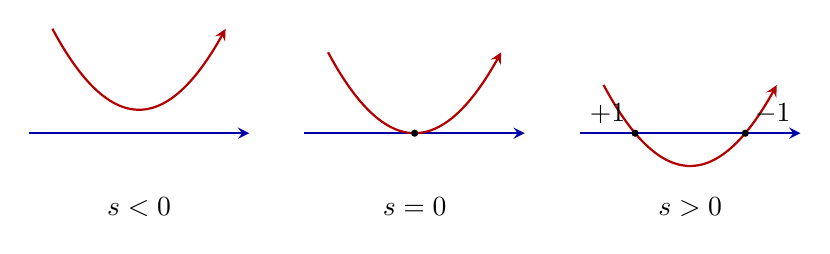
\begin{tikzpicture}[x=1cm,y=0.85cm,>=stealth]
	\begin{scope}
		\draw[->,blue!65!black,thick] (-1.4,0)--(1.4,0);
		\draw[->,red!70!black,thick,domain=-1.1:1.1,samples=40] plot (\x,{\x*\x+0.35});
		\node at (0,-1.1) {\(s<0\)};
	\end{scope}
	\begin{scope}[xshift=3.5cm]
		\draw[->,blue!65!black,thick] (-1.4,0)--(1.4,0);
		\draw[->,red!70!black,thick,domain=-1.1:1.1,samples=40] plot (\x,{\x*\x});
		\fill (0,0) circle (1.3pt);
		\node at (0,-1.1) {\(s=0\)};
	\end{scope}
	\begin{scope}[xshift=7cm]
		\draw[->,blue!65!black,thick] (-1.4,0)--(1.4,0);
		\draw[->,red!70!black,thick,domain=-1.1:1.1,samples=40] plot (\x,{\x*\x-0.49});
		\fill (-0.7,0) circle (1.3pt) node[above left] {\(+1\)};
		\fill (0.7,0) circle (1.3pt) node[above right] {\(-1\)};
		\node at (0,-1.1) {\(s>0\)};
	\end{scope}
\end{tikzpicture}

	\caption{相切附近的交点生成。曲线按横坐标递增定向，横轴向右定向；出现的两个交点分别贡献 \(+1\) 和 \(-1\)。}
	\label{g2:fig:intersection-pair}
\end{figure}

\subsection{一参数族给出的配边}
\label{g2:subsec:1602:03}

第14章已经将同伦横截化，得到连接端点逆像的紧流形。现在给这个配边定向，就能把模二不变性加强为整数不变性。这里需要核对时间方向与法方向的排列，而不只是指出端点成对出现。

\begin{theorem}\label{g2:thm:intersection-homotopy-invariance}
	设 \(M\) 是已定向、无边界的光滑 \(n\) 维流形，\(B\subset M\) 是已定向、闭的无边界嵌入 \(q\) 维子流形，\(X\) 是紧、已定向、无边界的光滑 \(p\) 维流形，\(p+q=n\)。若光滑映射 \(f_0,f_1:X\to M\) 横截于 \(B\) 且连续同伦，则
	\[
		I(f_0,B)=I(f_1,B).
	\]
\end{theorem}
\begin{proof}
	由\cref{g2:thm:transverse-homotopy-cobordism}，可选横截同伦 \(H:X\times[0,1]\to M\)，在两个端点的时间邻域中分别等于 \(f_0,f_1\)。其逆像 \(W=H^{-1}(B)\) 是紧一维带边界流形，边界是两端逆像的不交并。这里 \(X\) 紧、\(B\) 闭保证 \(W\) 紧。

	给 \(X\times[0,1]\) 取先 \(\mathrm{T}X\)、后 \(\partial_t\) 的乘积定向。商微分给出短正合列
	\[
		0\longrightarrow\mathrm{T}W\longrightarrow\mathrm{T}(X\times[0,1])|_W
		\xrightarrow{\ \overline{\mathrm{d}H}\ }H^*\nu B\longrightarrow0.
	\]
	规定 \(W\) 的正向，使法方向排在 \(W\) 的切方向之前，即 \((H^*\nu B,\mathrm{T}W)\) 给出源乘积的定向。更具体地，先列法基的提升，最后列 \(W\) 的正向切向量。

	在端点邻域，\(H\) 与时间无关。若 \(x\in f_i^{-1}(B)\)，记其局部符号为 \(\varepsilon_x\)。法基在 \(\mathrm{T}_xX\) 中的提升相对于 \(X\) 定向具有符号 \(\varepsilon_x\)，故上述规则使 \(W\) 的正向切向量为 \(\varepsilon_x\partial_t\)。采用外法向优先的边界定向，\(t=1\) 端点的符号是 \(\varepsilon_x\)，\(t=0\) 端点的符号是 \(-\varepsilon_x\)。因此
	\[
		\sum_{z\in\partial W}\varepsilon_z=I(f_1,B)-I(f_0,B).
	\]
	紧一维有向流形的边界符号之和为零：按第14章证明中的有限坐标弧分割，把各小弧沿定向排列，每条小弧贡献“终点减起点”，内部端点两两抵消，剩下的就是边界端点。于是右端为零。
\end{proof}

由此可对任意光滑 \(f:X\to M\) 选一个横截扰动 \(f'\)，定义 \(I(f,B)=I(f',B)\)。两个这样的扰动均与 \(f\) 同伦，定理保证良定义。对紧嵌入 \(A\) 使用上一小节的环境扰动，便定义 \(I_M(A,B)\)。其交换及反向规则仍成立：先把两片置于横截位置，再应用\cref{g2:prop:intersection-linear-signs}；更换所移动的一片也不影响结果，因为保持定向的环境微分同胚满足 \(I(A,\Phi(B))=I(\Phi^{-1}(A),B)\)，而 \(\Phi^{-1}|_A\) 与包含映射同伦。

\ProseParagraphBreak

紧性可以用“整个交点轨迹紧”替代，但不能只要求每张切片有有限个交点。例如 \(f_t:\mathbb R\to\mathbb R\)、\(f_t(x)=tx-1\)，以正向原点作为 \(B\)。\(t=0\) 时无交点，\(t>0\) 时恰有一个符号为正的交点 \(x=1/t\)。当 \(t\downarrow0\) 时它逃向无穷，轨迹不是紧配边，所以整数计数发生变化。这个例子说明，在非紧源上应用配边证明时，必须控制整条同伦的逆像。

\subsection{交数与帽积配对的比较}
\label{g2:subsec:1602:04}

以下设环境 \(M\) 闭且已定向，以便使用整数基本类 \([M]\)。\cref{g2:cor:closed-poincare-duality}给出同构
\[
	D_M:H^k(M;\mathbb Z)\longrightarrow H_{n-k}(M;\mathbb Z),\qquad
	D_M(\alpha)=\alpha\frown[M].
\]
对闭已定向嵌入子流形 \(i_B:B^q\hookrightarrow M\)，记
\[
	\mathrm{PD}_M(B)=D_M^{-1}\bigl((i_B)_*[B]\bigr)\in H^{n-q}(M;\mathbb Z).
\]
这里的 \(\mathrm{PD}\) 是 Poincaré 对偶类；它由帽积定义。要证明它检测穿过 \(B\) 的次数，需在 \(B\) 附近找到一个具体相对类，并核对其帽积正好留下 \(B\) 的基本类。

\begin{lemma}\label{g2:lem:normal-relative-class}
	设 \(M\) 是闭、已定向的光滑 \(n\) 维流形，\(B\subset M\) 是闭、已定向的嵌入 \(q\) 维子流形，\(p=n-q\)。法丛采用\eqref{g2:eq:normal-first-orientation}的定向。存在唯一的类
	\[
		u_B\in H^p(M,M\setminus B;\mathbb Z),
	\]
	使它在每个小法向 \(p\) 维盘上的限制，在正向局部基本类上取值 \(1\)。若 \(\overline u_B\) 是它在绝对上同调中的像，则
	\begin{equation}\label{g2:eq:normal-class-cap-fundamental}
		\overline u_B\frown[M]=(i_B)_*[B],\qquad
		\overline u_B=\mathrm{PD}_M(B).
	\end{equation}
\end{lemma}
\begin{proof}
	由\cref{g2:thm:tubular-neighborhood}，可将 \(B\) 的一个开邻域 \(U\) 识别为法丛的一个开圆盘丛；沿纤维径向重参数化，它与整个法丛 \(E\) 微分同胚，并保持零截面及纤维定向。\cref{g2:prop:relative-cohomology-exactness}的切除把 \(H^p(M,M\setminus B)\) 识别为 \(H^p(E,E\setminus B)\)。因此先在法丛中构造相对类。

	对任一法丛可平凡化的开集 \(V\subset B\)，选保持法向定向的平凡化，得到空间对
	\[
		(E|_V,E|_V\setminus V)\cong
		(\mathbb R^p\times V,(\mathbb R^p\setminus\{0\})\times V).
	\]
	相对 Eilenberg--Zilber 比较给出
	\begin{equation}\label{g2:eq:normal-low-degree-local}
		H^j(E|_V,E|_V\setminus V;\mathbb Z)\cong H^{j-p}(V;\mathbb Z).
	\end{equation}
	恢复这一计算的理由：\cref{g2:prop:cross-cup-evaluation}证明中的相对链比较将左侧链模型写成 \(C_*(\mathbb R^p,\mathbb R^p\setminus\{0\})\otimes C_*(V)\)。第一因子的同调只在 \(p\) 次为 \(\mathbb Z\)；由\cref{g2:lem:free-complex-splitting}，其圈边界序列可分裂为一个 \(\mathbb Z\) 加若干两项可缩复形，故它链同伦等价于仅在 \(p\) 次有 \(\mathbb Z\) 的复形。张量后再取 \(\operatorname{Hom}(-,\mathbb Z)\)，便得到上同调的次数平移。特别地，\(j<p\) 时左侧为零，\(j=p\) 时它由每个分支上的纤维取值唯一确定；全部取值为 \(1\) 的类就是正向纤维生成元与 \(1\in H^0(V)\) 的外积。

	这些局部类可以唯一粘合。取覆盖紧流形 \(B\) 的有限个丛平凡化开集，逐个取并。对两个开集 \(V,W\)，相对 Mayer--Vietoris 列包含
	\[
		H^{p-1}(E|_{V\cap W},E|_{V\cap W}\setminus(V\cap W))
		\longrightarrow H^p(E|_{V\cup W},E|_{V\cup W}\setminus(V\cup W))
	\]
	及其后的“限制到 \(V,W\)，再取交集上的差”两条箭头。这条列由相对小链模型的短正合列取对偶得到，和第6章使用的相对 Mayer--Vietoris 构造相同。归纳时，交集位于新加入的平凡化开集中，故\eqref{g2:eq:normal-low-degree-local}适用。其 \(p-1\) 次群为零，且两侧的 \(p\) 次局部类在交集上都以每根正向纤维的取值 \(1\) 为特征，所以差为零。正合性给出延拓的存在与唯一性。相同正合列也保持低于 \(p\) 次的消失，完成归纳。于是得到 \(u_B\)。改变管状邻域或平凡化后，纤维的局部取值不变，唯一性保证所取的是同一相对类。

	接着计算帽积。把 \(u_B\) 切除到 \(U\)，记作 \(u\)。\cref{g2:prop:relative-cap}给出
	\[
		z_U=u\frown[U]_B\in H_q(U;\mathbb Z),
	\]
	其中 \([U]_B\in H_n(U,U\setminus B;\mathbb Z)\) 是第6章的紧集基本类。令 \(r:U\to B\) 为管状收缩。要证明 \(r_*z_U=[B]\)，依\cref{g2:lem:compact-localization}，只需在每个 \(b\in B\) 核对其顶次局部值。

	在 \(b\) 附近选法向优先的乘积坐标 \((z,y)\in\mathbb R^p\times\mathbb R^q\)，其中 \(B\) 为 \(z=0\)。令 \(v_b\in H^q(B,B\setminus\{b\};\mathbb Z)\) 为在 \(B\) 的正向局部基本类上取值 \(1\) 的类。相对帽积的自然性及\eqref{g2:eq:cap-evaluation}在小链模型中的同一计算给出
	\begin{equation}\label{g2:eq:normal-cap-local-test}
		\left\langle v_b,\operatorname{loc}_b(r_*z_U)\right\rangle
		=\left\langle u\smile r^*v_b,[U]_{\{b\}}\right\rangle=1.
	\end{equation}
	说明这里的支集对应：\(u\) 的相对支集为 \(B\)，\(r^*v_b\) 的相对支集为法纤维 \(r^{-1}(b)\)，两者相交于 \(b\)。所以其相对杯积在 \(H^n(U,U\setminus\{b\})\) 中；局部化的基本类正是 \([U]_{\{b\}}\)。最后一个等号是\cref{g2:prop:local-cross-normalization}：先法向、后基底的两个正向局部生成元之积，在环境正向基本类上取值 \(1\)。某个因子为零维时，该计算退为点上乘法，结论相同。

	因此 \(r_*z_U\) 在每点的局部值都与 \([B]\) 相同，基本类的唯一性给出等式。将紧支相对类映入 \(M\)，帽积自然性又给出
	\[
		\overline u_B\frown[M]=(i_U)_*z_U
		=(i_B)_*r_*z_U=(i_B)_*[B].
	\]
	中间等式使用管状邻域沿纤维缩放到零截面的形变收缩。最后由 \(D_M\) 的单射性，\(\overline u_B=\mathrm{PD}_M(B)\)。
\end{proof}

这个相对类把“穿过 \(B\)”变成一个可以拉回的代数条件。法向小盘上的归一化决定每次横穿的贡献，上一证明中的帽积计算则保证它与第6章已经采用的对偶约定一致。

\begin{theorem}[几何相交与对偶配对]\label{g2:thm:geometric-intersection-pairing}
	设 \(M\) 是闭、已定向的光滑 \(n\) 维流形，\(B\subset M\) 是闭、已定向的嵌入 \(q\) 维子流形，\(X\) 是闭、已定向的光滑 \(p\) 维流形，\(p+q=n\)。若光滑映射 \(f:X\to M\) 横截于 \(B\)，且法丛采用法向优先定向，则
	\[
		\sum_{x\in f^{-1}(B)}\varepsilon_x(f,B)
		=\left\langle f^*\mathrm{PD}_M(B),[X]\right\rangle.
	\]
	对任意光滑 \(f\)，左侧采用横截扰动所定义的 \(I(f,B)\) 后，等式仍成立。特别地，若 \(A^p\subset M\) 也是闭已定向嵌入子流形，记 \([A]\)、\([B]\) 为其基本类在 \(M\) 中的推前，则
	\begin{equation}\label{g2:eq:intersection-cup-pairing}
		I_M(A,B)=\langle\mathrm{PD}_M(B),[A]\rangle
		=\langle\mathrm{PD}_M(A)\smile\mathrm{PD}_M(B),[M]\rangle.
	\end{equation}
\end{theorem}
\begin{proof}
	令 \(Z=f^{-1}(B)\)。它是有限点集。上一引理的相对类拉回为
	\[
		f^*u_B\in H^p(X,X\setminus Z;\mathbb Z).
	\]
	基本类的局部化与相对配对自然性给出
	\[
		\left\langle f^*\mathrm{PD}_M(B),[X]\right\rangle
		=\langle f^*u_B,[X]_Z\rangle
		=\sum_{x\in Z}\left\langle(f^*u_B)_x,[X]_x\right\rangle.
	\]
	最后一步在 \(Z\) 的互不相交小坐标邻域中切除；基本类限制到每点都为该点的正向局部类，所以有限直和中的每项系数都是 \(1\)。

	对 \(x\in Z\)，取 \(f(x)\) 附近的法向坐标 \(z:M\supset U\to\mathbb R^p\)。法向部分 \(z\circ f\) 在 \(x\) 的微分是定义 \(\varepsilon_x(f,B)\) 的线性同构。由逆函数定理，它在小邻域内为局部微分同胚，按其行列式符号将 \([X]_x\) 送到正向法盘基本类或其相反数。\(u_B\) 在这个正向法盘上取值 \(1\)，故每项恰等于 \(\varepsilon_x(f,B)\)。这证明横截情形。

	一般 \(f\) 的横截扰动 \(f'\) 与 \(f\) 同伦，所以它们诱导相同的上同调拉回；左侧按此前的不变性定义，等式随之成立。取 \(f=i_A\)，得到\eqref{g2:eq:intersection-cup-pairing}的第一个等式。第二个等式由帽积顺序决定：
	\[
		\begin{aligned}
		\langle\mathrm{PD}_M(B),[A]\rangle
		&=\langle\mathrm{PD}_M(B),\mathrm{PD}_M(A)\frown[M]\rangle\\
		&=\langle\mathrm{PD}_M(A)\smile\mathrm{PD}_M(B),[M]\rangle,
		\end{aligned}
	\]
	最后一行正是\eqref{g2:eq:cap-evaluation}。因此此处杯积先放 \(A\) 的对偶类，再放 \(B\) 的对偶类。
\end{proof}

\begin{corollary}\label{g2:cor:intersection-homological-invariance}
	闭已定向光滑 \(n\) 维流形中的互补维闭已定向嵌入子流形，其相交数只依赖整数同调类。它是这些类的双线性配对；若任一类为挠类，则相交数为零。交换两类乘以 \((-1)^{pq}\)，反转任一子流形或环境的定向均使相交数反号。
\end{corollary}
\begin{proof}
	\(D_M^{-1}\)、杯积及基本类取值均线性，所以\eqref{g2:eq:intersection-cup-pairing}只依赖同调类且双线性。若 \(r[A]=0\)，则 \(rI_M(A,B)=0\)，而整数群无挠，故 \(I_M(A,B)=0\)，另一因子同理。对偶类次数分别为 \(q,p\)，分次交换律给出 \((-1)^{pq}\)。子流形反向使其基本类及对偶类反号；环境反向使 \([M]\) 与 \(D_M\) 都反号，因此两个对偶类各反号，最终的基本类取值再反号，总变化仍为负号。
\end{proof}

\begin{example}\label{g2:exm:torus-poincare-sign-check}
	回到环面中的 \(a,b\)。令 \(\xi,\eta\in H^1(T^2;\mathbb Z)\) 分别从第一、第二圆周拉回正向生成元，则 \(\langle\xi\smile\eta,[T^2]\rangle=1\)。由帽积取值公式，\(D(\xi)=[b]\)、\(D(\eta)=-[a]\)，故
	\[
		\mathrm{PD}(a)=-\eta,\qquad \mathrm{PD}(b)=\xi,\qquad
		\langle(-\eta)\smile\xi,[T^2]\rangle=1.
	\]
	这与两条正向曲线的实际交点符号相同，也说明法向优先约定中的负号如何与杯积交换符号配合。
\end{example}

式\eqref{g2:eq:intersection-cup-pairing}也对任意互补维同调类定义代数相交配对；当类已有光滑子流形代表时，定理将它解释为横截交点数。以 \(\mathbb F_2\) 为系数时，同样的局部类、粘合与帽积证明给出模二相交配对：局部生成元没有正负之分，因而不需要环境及两片的整数定向。

% !TeX root = ../../Book2.tex
% 纲要标题：### 16.3 向量场零点指标
% 纲要位置：几何学计划纲要.md，第 1589 行。
% 正文状态：未撰写；本文件目前是框架。

% 纲要内容开始
% 
% * 局部球面映射度
% * 非退化零点的行列式符号
% * 局部扰动与指标可加性
% * Euler 类的后续解释
% 
% 纲要内容结束

\section{向量场零点指标}
\label{g2:sec:1603}

待撰写

\subsection{局部球面映射度}
\label{g2:subsec:1603:01}
待撰写

\subsection{非退化零点的行列式符号}
\label{g2:subsec:1603:02}
待撰写

\subsection{局部扰动与指标可加性}
\label{g2:subsec:1603:03}
待撰写

\subsection{Euler 类的后续解释}
\label{g2:subsec:1603:04}
待撰写
% 纲要条目排为编号小节标题，并进入目录与书签；说明段仍保留于纲要注释中。

% !TeX root = ../../Book2.tex
% 纲要标题：### 16.4 不动点与 Lefschetz 公式
% 纲要位置：几何学计划纲要.md，第 1646 行。
% 正文状态：未撰写；本文件目前是框架。

% 纲要内容开始
% 
% * 图像和对角线
% * 横截不动点的局部指数
% * 对角类和上同调迹
% * Lefschetz 数非零的存在推论
% 
% ---
% 
% 纲要内容结束

\section{不动点与 Lefschetz 公式}
\label{g2:sec:1604}

待撰写

\subsection{图像和对角线}
\label{g2:subsec:1604:01}
待撰写

\subsection{横截不动点的局部指数}
\label{g2:subsec:1604:02}
待撰写

\subsection{对角类和上同调迹}
\label{g2:subsec:1604:03}
待撰写

\subsection{Lefschetz 数非零的存在推论}
\label{g2:subsec:1604:04}
待撰写
% 纲要条目排为编号小节标题，并进入目录与书签；说明段仍保留于纲要注释中。


\begin{chaptersummary}
	映射度将每个正则原像的微分符号相加，所得整数既是推前基本类的倍数，也是拉回顶次形式的积分倍数。非紧源上，局部有限基本类和紧支形式承担相同的比较，而固有映射与整体固有同伦保证支集和无穷远处的控制。相交数用法向优先定向比较源切空间与目标法空间；横截扰动给出有限计数，有向一维配边保证它不依赖扰动，局部法向类进一步把它识别为帽积配对。

	\ProseParagraphBreak

	向量场的孤立零点由小球边界的方向度赋予指标，非退化时为线性化行列式的符号。保持边界无零的扰动只能重新分配内部指标，不能改变总和；闭流形上的截面同伦也保持总指标，即使流形不可定向。对于不动点，图像与对角线把同一局部度变成 \(\operatorname{sgn}\det(I-\mathrm{d}f_x)\)，对角类的杯积计算再把局部指数和化为 Lefschetz 数。非零总量迫使相应原像、交点或不动点存在，而总量为零仍可能有彼此抵消的局部贡献。
\end{chaptersummary}

\BookExercises

\begin{exercise}\label{g2:ex:degree-sublinear-perturbation}
	设 \(A\in\operatorname{GL}(n,\mathbb R)\)，\(r:\mathbb R^n\to\mathbb R^n\) 光滑，且 \(|r(x)|/|x|\to0\) 当 \(|x|\to\infty\)。证明 \(F(x)=Ax+r(x)\) 固有，计算其度，并证明 \(F\) 满射。若目标正则值的全部原像点处均有 \(\det\mathrm{D}F>0\)，这些原像点的数量有何限制？
\end{exercise}
\begin{solution}
	选 \(c>0\) 使 \(|Ax|\ge c|x|\)。在某个大球之外有 \(|r(x)|\le c|x|/2\)，所以同伦 \(H(x,t)=Ax+t r(x)\) 对所有 \(0\le t\le1\) 同时满足
	\[
		|H(x,t)|\ge c|x|/2.
	\]
	目标紧集有界，因而其在 \(H\) 下的原像包含于一个固定闭球与 \([0,1]\) 的乘积；该原像又闭，所以紧。因此 \(H\) 是整体固有同伦，特别 \(F\) 固有，且
	\[
		\deg F=\deg A=\operatorname{sgn}\det A\ne0.
	\]
	非零度给出满射性。若某正则值的全部原像符号为正，符号和就是原像点数。因原像非空，该数必须为1，同时迫使 \(\det A>0\)。若 \(\det A<0\)，任何正则值的原像都必须至少包含一个反向点。
\end{solution}

\begin{exercise}\label{g2:ex:proper-local-diffeomorphism-degree}
	设 \(f:M^n\to N^n\) 为连通定向无边界光滑流形间的固有光滑映射，\(n\ge1\)，且 \(\mathrm{d}f\) 处处可逆。证明 \(f\) 满射，所有纤维有同一个有限正基数 \(r\)，并有 \(|\deg f|=r\)。若某个纤维只有一个点，证明 \(f\) 为微分同胚。将此结论用于上一题：若 \(\det\mathrm{D}F\) 处处非零，可以得到什么加强？
\end{exercise}
\begin{solution}
	微分的定向符号是 \(M\) 上连续取值于 \(\{1,-1\}\) 的函数，因连通性而恒等于某个 \(\varepsilon\)。任取 \(x_0\in M\)，\(y_0=f(x_0)\) 是正则值，紧离散纤维有有限个 \(r_0\ge1\) 点。因此 \(\deg f=\varepsilon r_0\ne0\)，从而 \(f\) 满射。所有目标点都是正则值，再次使用求和公式，得到
	\[
		\deg f=\varepsilon\#f^{-1}(y),
	\]
	所以每个纤维都有 \(r_0=|\deg f|\) 个点。若某个纤维单点，则全部纤维单点，\(f\) 双射。它的局部逆由逆函数定理光滑；各局部逆在交叠处因单射性一致，故拼成光滑整体逆。

	上一题已给出 \(|\deg F|=1\)，因此若 \(\mathrm{D}F\) 处处可逆，\(F:\mathbb R^n\to\mathbb R^n\) 就是整体微分同胚。这里无穷远处的增长控制与局部微分可逆分别保证固有性与局部逆，两者合起来才得到整体逆。
\end{solution}

\begin{exercise}\label{g2:ex:real-polynomial-degree}
	设 \(p(x)=a_mx^m+\cdots+a_0\) 是非常数实多项式，\(a_m\ne0\)。把实线取标准定向，按 \(m\) 的奇偶性及 \(a_m\) 的符号计算 \(\deg p\)。由此证明：对任意正则值 \(y\)，方程 \(p(x)=y\) 的实根数与 \(m\) 模2同余。证明中须核对所用同伦的整体固有性。
\end{exercise}
\begin{solution}
	令 \(q(x)=p(x)-a_mx^m\)，取同伦 \(H(x,t)=a_mx^m+tq(x)\)。因 \(\deg q<m\)，充分大 \(|x|\) 时有 \(|q(x)|\le|a_m||x|^m/2\)，故
	\[
		|H(x,t)|\ge |a_m||x|^m/2
	\]
	对所有 \(t\in[0,1]\) 同时成立。与上一题同理，\(H\) 整体固有，因而 \(\deg p=\deg(x\mapsto a_mx^m)\)。

	若 \(m\) 为奇数，任取非零目标值，有唯一实原像，导数 \(ma_mx^{m-1}\) 的符号为 \(\operatorname{sgn}a_m\)，故度为该符号。若 \(m\) 为偶数，取与 \(a_m\) 异号的目标值，原像为空，故度为0。等价地，同号非零目标值的两个原像导数符号相反，仍给出0。

	正则值的所有实原像都是单根，且有限。模2后每个 \(\pm1\) 都等于1，所以
	\[
		\#p^{-1}(y)\equiv\deg p\equiv m\pmod2.
	\]
	这既给出奇次多项式至少有一个实根，也说明偶次情形的正则实根总数为偶数。
\end{solution}

\begin{exercise}\label{g2:ex:boundary-degree-balance}
	设 \(W^{n+1}\) 为紧定向光滑带边界流形，\(n\ge1\)，边界的连通分支为 \(M_1,\ldots,M_s\)，均取外法向优先定向。设 \(N^n\) 为连通闭定向光滑流形，\(F:W\to N\) 光滑，记 \(f_j=F|_{M_j}\)。证明
	\[
		\sum_{j=1}^s\deg f_j=0.
	\]
	把结论用于圆环 \(W=\{z\in\mathbb C:1\le|z|\le2\}\)：若把内、外两个边界圆都按逆时针方向参数化，它们到 \(S^1\) 的限制映射度是什么关系？
\end{exercise}
\begin{solution}
	取 \(N\) 上积分为1的光滑顶次形式 \(\eta\)。因为 \(\mathrm{d}\eta=0\)，第一卷的 Stokes 定理和\cref{g2:thm:degree-comparison}给出
	\[
		\sum_j\deg f_j
		=\sum_j\int_{M_j}f_j^*\eta
		=\int_{\partial W}F^*\eta
		=\int_W\mathrm{d}(F^*\eta)=0.
	\]
	关键是所有边界分支使用诱导定向。对平面标准定向的圆环，外边界的诱导方向为逆时针，内边界为顺时针。因此若两个参数圆都取逆时针方向，内边界度要在上述和式中另乘 \(-1\)。公式成为 \(\deg f_{\mathrm{out}}-\deg f_{\mathrm{in}}=0\)，即二者的度相等。单边界情形的延拓障碍可对照\cite[第459页，定理17.38]{Lee2012Smooth}。
\end{solution}

% 第16.2节习题候选，题目及解答供并入章末。
\begin{exercise}\label{g2:ex:torus-slope-intersection}
	给 \(T^2=\mathbb R^2/\mathbb Z^2\) 取标准定向。设 \((r,s),(u,v)\in\mathbb Z^2\) 均为非零本原向量，令 \(A(t)=(rt,st)\)、\(B(t)=(ut,vt)\)，参数 \(t\) 模 \(1\)，并以递增参数定向。证明这两条曲线为嵌入圆周，且 \(I(A,B)=rv-su\)。当 \(rv-su\ne0\) 时求实际交点数；当 \(rv-su=0\) 时给出不交的微小扰动。
\end{exercise}
\begin{solution}
	若 \(A(t)=A(t')\)，则 \(r(t-t'),s(t-t')\in\mathbb Z\)。由 Bézout 等式及 \(\gcd(r,s)=1\)，得 \(t-t'\in\mathbb Z\)，故 \(A\) 单射；其导数不为零，源紧，所以为嵌入，\(B\) 同理。记标准坐标圆周类为 \(a,b\)，则 \([A]=ra+sb\)、\([B]=ua+vb\)。正文已算出 \(I(a,b)=1\)、\(I(b,a)=-1\)；平移一个坐标圆周得到与原圆周不交的同调代表，所以 \(I(a,a)=I(b,b)=0\)。双线性给出 \(I(A,B)=rv-su\)。

	还可直接数交点。取整数矩阵 \(P\in\operatorname{SL}(2,\mathbb Z)\)，使 \(P(r,s)^{\mathsf T}=(1,0)^{\mathsf T}\)；它由 Bézout 等式构造，并诱导保持定向的环面微分同胚。记 \(P(u,v)^{\mathsf T}=(u',v')^{\mathsf T}\)，则 \(v'=rv-su\)。\(B\) 与水平圆周相交恰要求 \(v't\in\mathbb Z\)。若 \(v'\ne0\)，模 \(1\) 恰有 \(|v'|\) 个参数；\(B\) 嵌入，给出相同数量的不同交点。各点的有序切向量行列式均为 \(v'\)，所以全部具有符号 \(\operatorname{sgn}(v')\)。若 \(v'=0\)，本原性使 \(u'=\pm1\)，两曲线的像都是水平圆周；将其中一条平移到 \(y=\varepsilon\ne0\) 即不相交，再用 \(P^{-1}\) 送回即可。
\end{solution}

\begin{exercise}\label{g2:ex:product-sphere-self-intersection}
	给 \(S^2\times S^2\) 取先第一因子、后第二因子的乘积定向。令 \(A=S^2\times\{y_0\}\)、\(B=\{x_0\}\times S^2\)，分别取因子定向。计算它们的全部相交配对。若闭已定向嵌入曲面 \(\Sigma\subset S^2\times S^2\) 满足 \([\Sigma]=m[A]+n[B]\)，求 \(I(\Sigma,\Sigma)\)，并说明 \(mn\ne0\) 时为何任何与 \(\Sigma\) 同调的嵌入曲面都不能与它不交。
\end{exercise}
\begin{solution}
	两片在 \((x_0,y_0)\) 唯一相交，先列 \(A\) 的正向基、再列 \(B\) 的正向基，正好是乘积正向基，所以 \(I(A,B)=1\)。两片维数均为 \(2\)，交换符号为 \((-1)^4=1\)，故 \(I(B,A)=1\)。把 \(y_0\) 移到另一点，得到与 \(A\) 同调且不交的纤维，故 \(I(A,A)=0\)；同理 \(I(B,B)=0\)。于是交矩阵为
	\[
		\begin{pmatrix}0&1\\1&0\end{pmatrix},\qquad
		I(\Sigma,\Sigma)=2mn.
	\]
	如果 \(\Sigma'\) 与 \(\Sigma\) 同调且二者不交，则 \(I(\Sigma,\Sigma')=0\)。同调不变性却使该数等于 \(2mn\)，所以 \(mn\ne0\) 时不可能。这里的自交数按两份代表作横截扰动计算，并非把 \(\Sigma\cap\Sigma\) 当成有限点集。
\end{solution}

\begin{exercise}\label{g2:ex:intersection-boundary-sign}
	设 \(M^n\) 是已定向无边界光滑流形，\(C^{p+1}\subset M\) 是紧已定向带边界嵌入子流形，\(A=\partial C\) 采用外法向优先的边界定向，\(B^q\subset M\) 是已定向闭嵌入无边界子流形，\(p+q=n\)。假设 \(C\) 及 \(A\) 都与 \(B\) 横截。用一维交集 \(W=C\cap B\) 证明 \(I(A,B)=0\)，并计算 \(\partial W\) 的点符号与 \(\varepsilon_z(A,B)\) 的关系，其中 \(W\) 按 \((\nu B,\mathrm{T}W)=\mathrm{T}C\) 定向。
\end{exercise}
\begin{solution}
	带边界横截逆像定理给出紧一维流形 \(W\)，并有 \(\partial W=A\cap B\)。设 \(z\) 为边界交点，\(a_1,\ldots,a_p\) 是 \(A\) 的正向基，\(o\) 是 \(C\) 的向外方向，则 \((o,a_1,\ldots,a_p)\) 给出 \(C\) 的正向。因为 \(A\pitchfork B\)，法基可在 \(\mathrm{T}A\) 内提升；其相对于 \((a_1,\ldots,a_p)\) 的符号为 \(\varepsilon_z(A,B)\)。

	把 \(o\) 从这些法基提升之后移到之前，需要交换 \(p\) 次。因而将 \(W\) 的正向与它的向外方向比较，得到
	\[
		\varepsilon_z(\partial W)=(-1)^p\varepsilon_z(A,B).
	\]
	向外向量为使其切于 \(W\) 而添加的切向分量，不改变这一行列式符号。紧一维有向流形的边界符号之和为零，故
	\[
		0=\sum_{z\in\partial W}\varepsilon_z(\partial W)=(-1)^pI(A,B),
	\]
	即 \(I(A,B)=0\)。
\end{solution}

\begin{exercise}\label{g2:ex:projective-lines-mod-two-intersection}
	在 \(\mathbb RP^2\) 中取两条不同的射影直线 \(L_0,L_1\)。证明它们横截相交于一点，模二相交数为 \(1\)，因而与它们分别模二同调的两个嵌入圆周不能不交。解释为何不能在本例中直接使用本节的整数有向相交配对。
\end{exercise}
\begin{solution}
	射影直线来自 \(\mathbb R^3\) 中的二维线性子空间。两个不同二维子空间的交恰为一维，所以对应的射影直线只有一个交点。作线性坐标变换后，可设它们分别为 \(z_2=0\) 和 \(z_1=0\)，交点为 \([1:0:0]\)。在仿射图 \(z_0\ne0\) 中，两条直线是两个坐标轴，故横截。模二计数因此为 \(1\)。

	本节模二版本的几何相交与对偶配对说明该数只依赖模二同调类。若两条相应代表不交，计数就为 \(0\)，与 \(1\) 矛盾。\(\mathbb RP^2\) 不可定向，且直线的法线丛也是不可定向的：把一条直线提升为 \(S^2\) 上的赤道，沿赤道的一个固定向北法向量在对径识别下被微分送到相反方向，绕投影圆周一周后法向反转。因此本例不能连续选择整数局部符号所需的法向定向，而模二计数不受反号影响。
\end{solution}

\begin{exercise}\label{g2:ex:mixed-monomial-vector-index}
	在标准平面切标架中，把向量场的系数写成复数。设它在原点附近满足
	\[
		F(z)=z^p\overline z^{\,q}+r(z),\qquad r(z)=o(|z|^{p+q}),
	\]
	其中 \(p,q\ge0\)、\(p+q\ge1\)，且 \(F\) 光滑。证明原点是孤立零点，指标为 \(p-q\)。在充分小的闭圆盘内，将该场作一个在边界上充分小的扰动，假设新场全部零点非退化。证明新零点总数 \(N\) 满足
	\[
		N\ge|p-q|,\qquad N\equiv p-q\pmod2.
	\]
\end{exercise}
\begin{solution}
	令 \(d=p+q\)。充分小的 \(|z|>0\) 时，\(|r(z)|<|z|^d/2\)，而 \(|z^p\overline z^{\,q}|=|z|^d\)，所以 \(|F(z)|>|z|^d/2>0\)。同时 \(F(0)=0\)，故原点孤立。对 \(0\le s\le1\)，\(z^p\overline z^{\,q}+s r(z)\) 在这个穿孔邻域内都非零。边界归一化因此把 \(F\) 同伦到主项；在 \(z=\varepsilon e^{\mathrm i\theta}\) 上，主项的单位方向为 \(e^{\mathrm i(p-q)\theta}\)。圆周映射度于是给出 \(\operatorname{ind}_0(F)=p-q\)。

	固定上述小圆盘 \(D\)，记 \(c=\min_{\partial D}|F|>0\)。若扰动 \(G\) 满足 \(\sup_{\partial D}|G-F|<c\)，则 \((1-s)F+sG\) 在边界始终非零。新零点集闭且不碰边界，非退化性又使它离散，故有限。记正、负指标零点数为 \(N_+,N_-\)。由\cref{g2:thm:local-index-additivity,g2:prop:nondegenerate-vector-index}，
	\[
		N_+-N_-=p-q,\qquad N=N_++N_-.
	\]
	因此 \(N\ge|p-q|\)，且 \(N-(p-q)=2N_-\)，得到奇偶约束。当 \(p=q\) 时原零点仍孤立，但指标为零，结论只要求扰动后的非退化零点成偶数出现，允许全部消失。
\end{solution}

\begin{exercise}\label{g2:ex:product-vector-field-index}
	设 \(X\) 是 \(m\) 维无边界光滑流形 \(M\) 上的向量场，\(Y\) 是 \(n\) 维无边界光滑流形 \(N\) 上的向量场，\(m,n\ge1\)。若 \(a,b\) 分别是其孤立零点，定义乘积场 \(Z(x,y)=(X(x),Y(y))\)。用局部相对同调外积的自然性证明
	\[
		\operatorname{ind}_{(a,b)}Z=\operatorname{ind}_aX\operatorname{ind}_bY.
	\]
	对 \(\mathbb R^3=\mathbb C\times\mathbb R\) 上系数为 \((z^k,-t)\) 的场，\(k\ge1\)，计算原点指标。
\end{exercise}
\begin{solution}
	取把 \(a,b\) 移到零点的坐标，系数分别为 \(F:U\to\mathbb R^m\)、\(G:V\to\mathbb R^n\)，并缩小 \(U,V\)，使每个映射仅在原点为零。乘积系数 \(F\times G\) 在 \(U\times V\) 中也只在 \((0,0)\) 为零，所以乘积零点孤立。

	记正向局部同调生成元为 \(\mu_m,\mu_n\)。第4章相对外积的自然性适用于穿孔开集，因为
	\[
		(U\setminus\{0\})\times V\ \cup\ U\times(V\setminus\{0\})
		=(U\times V)\setminus\{(0,0)\}.
	\]
	\cref{g2:prop:local-cross-normalization}证明中的定向乘积链说明，先列 \(U\) 坐标、再列 \(V\) 坐标时，\(\mu_m\times\mu_n=\mu_{m+n}\)，没有额外符号。于是
	\begin{align*}
		(F\times G)_*(\mu_m\times\mu_n)
		&=F_*\mu_m\times G_*\mu_n\\
		&=(\deg_0F)(\deg_0G)(\mu_m\times\mu_n).
	\end{align*}
	\cref{g2:prop:vector-index-well-defined}已将系数映射的局部同调度识别为向量场指标，因此得到乘法公式。此论证同时适用于退化零点，不要求微分可逆。

	在 \(\mathbb C\) 因子，\(z^k\) 的原点指标为 \(k\)；在实线因子，\(-t\) 的指标为 \(-1\)。采用坐标顺序 \((\operatorname{Re}z,\operatorname{Im}z,t)\)，乘积指标为 \(-k\)。
\end{solution}

\begin{exercise}\label{g2:ex:punctured-rotating-frame-index}
	在穿孔平面圆盘中写 \(z=r e^{\mathrm i\theta}\)，对整数 \(k\) 取由标准标架转动 \(k\theta\) 得到的正向标架
	\[
		e_1=(\cos k\theta,\sin k\theta),\qquad
		e_2=(-\sin k\theta,\cos k\theta).
	\]
	求径向场 \(X(x,y)=(x,y)\) 在这组标架中的系数沿小圆周的绕数。证明当 \(k\ne0\) 时，这组标架不能作为处处非退化的连续标架延过原点，并说明所得系数绕数为什么不违背局部指标的坐标无关性。
\end{exercise}
\begin{solution}
	把平面向量写成复数时，标架变换就是乘以 \(e^{\mathrm ik\theta}\)。若 \(c\) 表示径向场在新标架中的复系数，则 \(e^{\mathrm ik\theta}c=r e^{\mathrm i\theta}\)，所以
	\[
		c=r e^{\mathrm i(1-k)\theta}.
	\]
	沿小圆周归一化后，其绕数为 \(1-k\)。

	若该标架能非退化地连续延过原点，第一列向量 \(e_1\) 就在整个小闭圆盘上连续且非零。将它归一化，可得从闭圆盘到 \(S^1\) 的连续映射，其边界限制为 \(e^{\mathrm i\theta}\mapsto e^{\mathrm ik\theta}\)。把边界圆沿径向缩到圆心，得到这一映射与常值映射的同伦，故边界度必须为0。但它的度为 \(k\)，所以 \(k\ne0\) 时不可能延拓。

	向量场指标要求使用包含零点的坐标图及其坐标切标架。这里 \(k\ne0\) 的标架只存在于穿孔圆盘，零点处缺少这份坐标识别，故不能用其系数绕数代替原点指标。标准标架中的径向场指标仍为1；差出的 \(k\) 正是沿圆周旋转标架自身所贡献的绕数。
\end{solution}

\begin{exercise}\label{g2:ex:odd-dimensional-total-index}
	设 \(X\) 是无边界光滑 \(n\) 维流形上的向量场，\(n\ge1\)，\(p\) 是孤立零点。证明
	\[
		\operatorname{ind}_p(-X)=(-1)^n\operatorname{ind}_pX.
	\]
	再仅用本章的总指标不变性，证明奇数维闭流形上任何只有孤立零点的光滑向量场，其总指标为零；因此它不可能恰有一个零点且该零点非退化。若所有零点都非退化，正、负指标零点数有何关系？
\end{exercise}
\begin{solution}
	在零点附近写 \(X\) 的系数为 \(F\)。负场的单位方向映射为 \(a\circ\widehat F\)，其中 \(a:S^{n-1}\to S^{n-1}\)、\(a(u)=-u\)。\cref{g2:prop:reflection-antipodal-degree}给出 \(\deg a=(-1)^n\)，复合公式遂得所求恒等式。\(n=1\) 时 \(a\) 交换 \(S^0\) 的两点，在约化零次同调上乘以 \(-1\)，同样成立。

	现设 \(M\) 闭且 \(n\) 为奇数。零点集有限，且 \(X,-X\) 有相同零点。记 \(J=\sum_p\operatorname{ind}_pX\)。\cref{g2:thm:total-vector-index-invariance}使 \(-X\) 的总指标也为 \(J\)，而逐点的公式又使它等于 \(-J\)。所以 \(2J=0\)；\(J\) 为整数，故 \(J=0\)。这里不需要整体定向，也没有使用指标总和与 Euler 示性数的比较。

	单个非退化零点的指标为 \(\pm1\)，无法构成总和0，因此题述情形不可能。若所有零点都非退化，设其正、负指标数为 \(N_+,N_-\)，则 \(N_+-N_-=J=0\)，所以两类数量相同，零点总数为偶数。
\end{solution}

\begin{exercise}\label{g2:ex:torus-affine-lefschetz}
	设 \(A\in M_2(\mathbb Z)\)、\(b\in\mathbb R^2\)，令 \(f:\mathbb R^2/\mathbb Z^2\to\mathbb R^2/\mathbb Z^2\) 为 \(f([x])=[Ax+b]\)。计算 \(L(f)\)。若 \(\det(I-A)\ne0\)，证明它恰有 \(|\det(I-A)|\) 个不动点，并计算每点指数。
\end{exercise}
\begin{solution}
	平移 \(b\) 可通过 \(tb\) 同伦移去。一次同调上的矩阵为 \(A\)，一次上同调上的矩阵为 \(A^{\mathsf T}\)；零次作用为恒等，二次作用为乘 \(\det A\)。因此
	\[
		L(f)=1-\operatorname{tr}A+\det A=\det(I-A).
	\]
	记 \(B=I-A\)。不动点方程是 \(Bx\equiv b\pmod{\mathbb Z^2}\)。若 \(\det B\ne0\)，先取 \(x_0=B^{-1}b\)，全部解在环面上形成陪集 \([x_0]+\ker\overline B\)。核为 \(B^{-1}\mathbb Z^2/\mathbb Z^2\)，乘以 \(B\) 将其同构到 \(\mathbb Z^2/B\mathbb Z^2\)。整数 Smith 标准形将后者写成两个有限循环群的直和，其阶为两个非零对角因子的绝对值之积，即 \(|\det B|\)。每点微分均为 \(A\)，故均非退化，指数都等于 \(\operatorname{sgn}\det B\)。指数和为 \(|\det B|\operatorname{sgn}\det B=\det B\)，与 \(L(f)\) 一致。
\end{solution}

\begin{exercise}\label{g2:ex:even-complex-projective-fixed-point}
	设 \(r\geq1\)。利用 \(H^*(\mathbb CP^{2r};\mathbb Z)=\mathbb Z[u]/(u^{2r+1})\)、\(|u|=2\)，证明每个连续映射 \(f:\mathbb CP^{2r}\to\mathbb CP^{2r}\) 都有不动点。\cite[第2.C节，The Lefschetz Fixed Point Theorem]{Hatcher2002}
\end{exercise}
\begin{solution}
	二次整数上同调由 \(u\) 生成，故 \(f^*u=du\)，其中 \(d\in\mathbb Z\)。拉回保持杯积，所以 \(f^*(u^k)=d^ku^k\)。只有偶次上同调非零，故
	\[
		L(f)=1+d+d^2+\cdots+d^{2r}.
	\]
	若 \(d\geq0\)，这个和至少为 \(1\)。若 \(d\leq-1\)，则
	\[
		1+d+\cdots+d^{2r}=\frac{d^{2r+1}-1}{d-1}>0,
	\]
	因为分子、分母同为负数。于是对所有整数 \(d\) 都有 \(L(f)>0\)，由 Lefschetz 不动点定理得到结论。证明使用了杯积将二次作用与所有高偶次作用联系起来，单独知道各次群的秩还不足以得到这些幂次关系。
\end{solution}

\begin{exercise}\label{g2:ex:lefschetz-product}
	设 \(M,N\) 是闭、已定向光滑流形，\(f:M\to M\)、\(g:N\to N\) 连续。证明 \(L(f\times g)=L(f)L(g)\)。如果两映射都光滑且全部不动点非退化，再用局部指数给出同一等式的几何证明。
\end{exercise}
\begin{solution}
	有限维上同调的 Künneth 同构将 \(H^k(M\times N;\mathbb R)\) 写为 \(\bigoplus_{p+q=k}H^p(M;\mathbb R)\otimes H^q(N;\mathbb R)\)。由外积自然性，\((f\times g)^*\) 在对应直和项上为 \(f^*\otimes g^*\)。若两矩阵为 \(A,B\)，则张量基中对角元为 \(A_{ii}B_{jj}\)，所以 \(\operatorname{tr}(A\otimes B)=\operatorname{tr}A\operatorname{tr}B\)。因此
	\[
		L(f\times g)=\sum_{p,q}(-1)^{p+q}\operatorname{tr}(f^*|_{H^p(M)})\operatorname{tr}(g^*|_{H^q(N)})=L(f)L(g).
	\]
	在非退化情形，不动点集为两个有限不动点集的乘积。微分是块对角矩阵，故
	\[
		\operatorname{ind}(f\times g,(x,y))
		=\operatorname{sgn}\det(I-\mathrm{d}f_x)\operatorname{sgn}\det(I-\mathrm{d}g_y).
	\]
	分别对 \(x,y\) 求和，再用 Lefschetz 公式，便得同一等式。
\end{solution}

\begin{exercise}\label{g2:ex:degenerate-circle-fixed-indices}
	固定 \(0<\varepsilon<1/4\)，在 \(S^1=\mathbb R/\mathbb Z\) 上定义 \(f([t])=[t+\varepsilon\sin^2(2\pi t)]\)。求全部不动点及其指数。再考虑 \(f_a([t])=[t+\varepsilon\sin^2(2\pi t)-a]\)：当 \(0<a<\varepsilon\) 时求不动点个数和指数，并说明当 \(-\varepsilon<a<0\) 时发生了什么。
\end{exercise}
\begin{solution}
	\(f\) 的位移增量在 \([0,\varepsilon]\subset[0,1)\) 内，所以不动点恰为 \([0]\)、\([1/2]\)。各点附近的 \(t-f(t)=-\varepsilon\sin^2(2\pi t)\) 在两侧都为负，故由一维局部指数公式，两点指数都为零。所有 \(f_a\) 都同伦于恒等映射，所以 \(L(f_a)=0\)。

	若 \(0<a<\varepsilon\)，位移增量位于 \((-1,1)\)，不动点方程恰为 \(\sin^2(2\pi t)=a/\varepsilon\)。一个周期内有四个解，每个原不动点两侧各有一个。局部位移为 \(h_a(t)=a-\varepsilon\sin^2(2\pi t)\)，其导数
	\[
		h_a'(t)=-4\pi\varepsilon\sin(2\pi t)\cos(2\pi t)
	\]
	在四个解处均非零，符号依次交替；围绕每个原不动点的两个指数分别为 \(+1\)、\(-1\)，故各小邻域内的总指数仍为零。若 \(-\varepsilon<a<0\)，增量 \(\varepsilon\sin^2(2\pi t)-a\) 严格位于 \((0,2\varepsilon)\subset(0,1)\)，没有不动点。原来的两个零指数不动点因此都可在小扰动下消失。
\end{solution}
